\documentclass[11pt]{article}
\usepackage{geometry}
 \geometry{
 a4paper,
 total={170mm,257mm},
 left=20mm,
 top=20mm,
 }
%Gummi|065|=)
\title{\textbf{CS747 - Assignment 4}}
\author{Kalpesh Krishna\\140070017\\kalpeshk2011@gmail.com}
\date{}
\usepackage{graphicx}
\begin{document}

\maketitle

\section{Implementation \& Results}
All algorithms were implemented in Python without the use of any external library except \texttt{numpy} to generate random numbers and carry out matrix updates. The \texttt{weights} array has been offset by 1 to start indices from 1 (instead of 0) to match Baird's counterexample diagram. A random seed 0 has been used in all experiments.
\subsection{Experiment 1}
In this experiment, all non-terminal states are chosen in a round robin fashion followed by a TD($0$) style update. The figure below shows the graph obtained. This is similar in shape to the graph obtained in chapter 8 of Sutton and Barto 1998.
\begin{center}
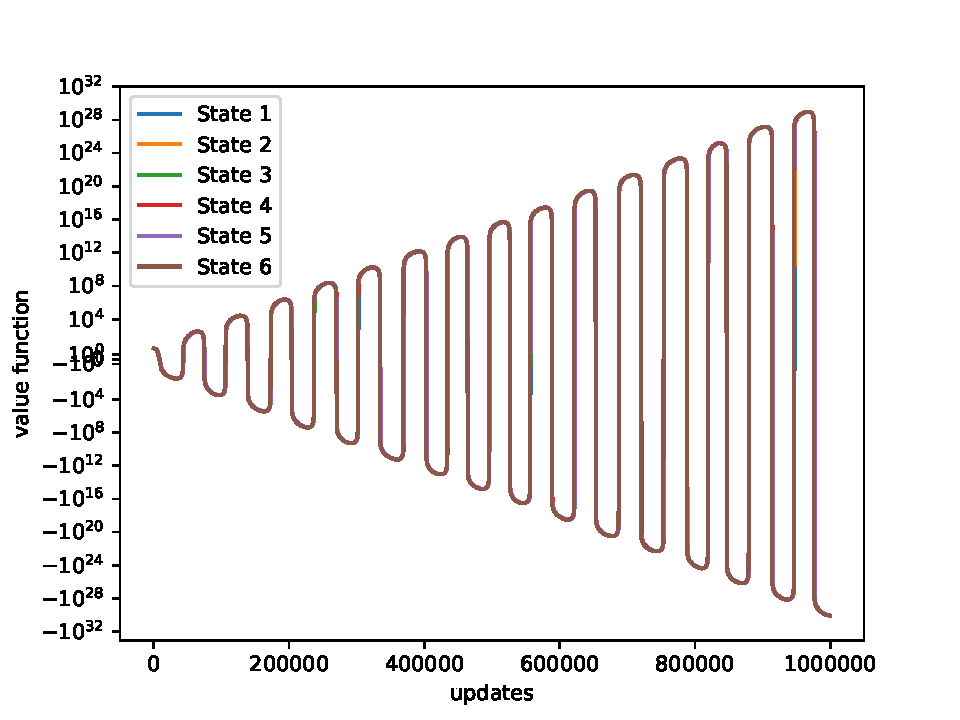
\includegraphics[width=15cm]{expt1.pdf}
\end{center}
\textbf{Explanation} - To analyse this system, we first plot a graph between the weight values and the corresponding number of iterations (shown below). Quite clearly, $w[7]$ updates faster than $w[1..5]$. (since it is updated 5 times for every update of $w[1..5]$. The weight $w[6]$ updates the slowest, since 99\% of the time it self loops and the update is just due to $\gamma$. After a point, the value of $V(6)$ is higher than each of $V(1..5)$, (since $w[6]$ is still positive at this point) causing the weights in state $1..5$ to start increasing and $w[6]$ to start decreasing. This cycle and osscillation of weights continues with increase in number of iterations. This system is an unstable system (as described in Sutton and Barto) and hence value functions diverge. 
\begin{center}
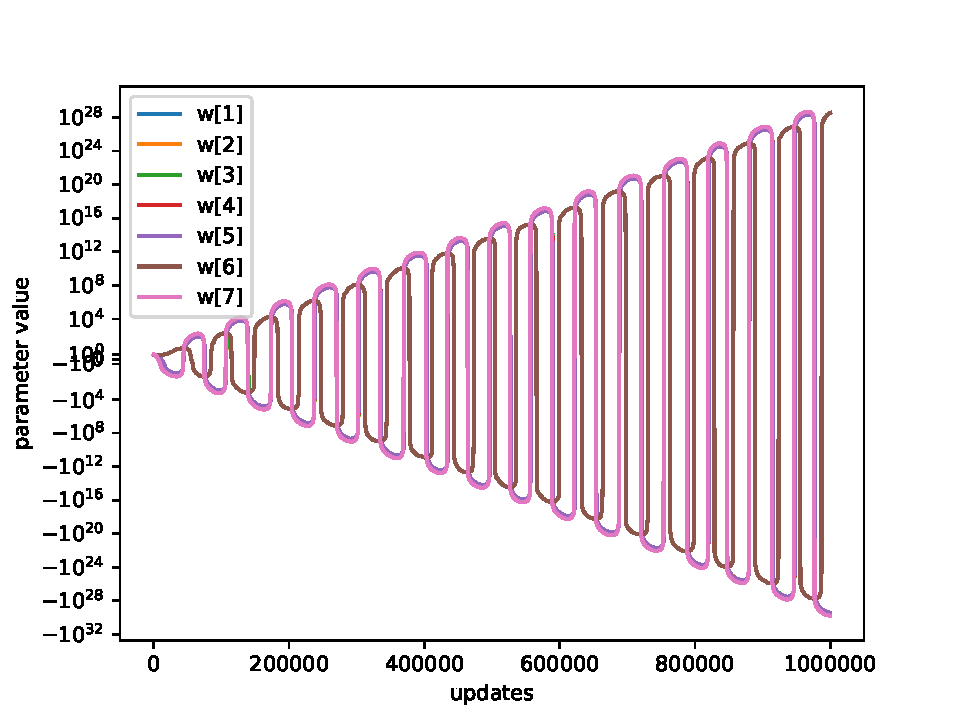
\includegraphics[width=15cm]{expt1_2.pdf}
\end{center}

\subsection{Experiment 2}
No significant difference was observed by changing the value of $\lambda$. Unlike the previous case, $V[1...5]$ are updated less often. $w[1...5]$ are updated exactly once for each significant update in $w[6]$ in the TD(0) case. In the previous task, $w[6]$ undergoes a significant update roughly once in 600 iterations, whereas $w[1...5]$ are updated 100 times each. (note that we are calling $\gamma V(6) - V(6)$ ``insignificant'' here).
\begin{center}
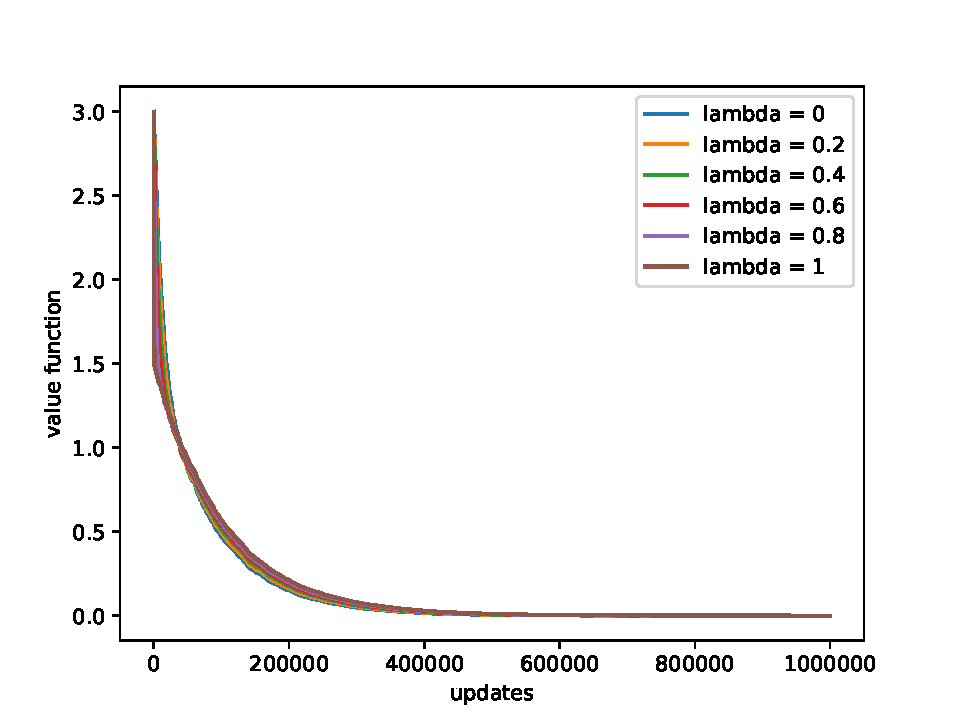
\includegraphics[width=15cm]{expt2.pdf}
\end{center}
\subsection{Experiment 3}
I noticed that changing the initial set of weights did not affect the final value function achieved. However, some configurations were taking longer to converge, which I suspect is due to a constant learning rate. The final set of weights were different, they differed by a constant factor. However, the ratio of $w[1...5] : w[6] : w[7]$ was always roughly $1:4:-2$, which is expected behavior due to the choice of function approximation. Raw output has been added below. \\
\begin{verbatim}
./startmdp.sh 2 1000000 0 1 1 1 1 1 1 1
Weights
[ 0.27999309  0.28000883  0.28002641  0.28001831  0.2799872   1.11999228
 -0.55999853]
Value Function
-1.23541347308e-05 1.91397635615e-05 5.42867724099e-05 3.8093030442e-05 -2.4125545401e-05 -4.77379483987e-06
./startmdp.sh 2 1000000 0 3 1 10 1 10 1 2
Weights
[ 0.99940458  0.99880368  1.00166754  0.9984671   1.00126741  4.00009876
 -1.99999732]
Value Function
-0.0011881549616 -0.00238995587097 0.00333776830031 -0.00306312343532 0.00253750595343 0.000104130358785 
./startmdp.sh 2 1000000 0 100 1 0 1 4 80 3
Weights
[ 16.82400073  16.79381982  16.79406201  16.79204024  16.79566909
  67.20004989 -33.60010428]
Value Function
0.0478971806153 -0.0124646358046 -0.0119802537092 -0.0160238019396 -0.0087660968456 -0.00015866026969 
./startmdp.sh 2 1000000 0 1000 1 0 1 4 80 3
Weights
[  53.04225399   52.73819236   52.74732618   52.72276639   52.74817208
  211.19984362 -105.60095726]
Value Function
0.483550712958 -0.124572552079 -0.106304900622 -0.1554244781 -0.104613113732 -0.00207090789942 
./startmdp.sh 2 1000000 0 1000 1 0 1 4 800 3
Weights
[ 168.24305459  167.93828292  167.94312627  167.92048556  167.95005989
  672.00069251 -336.00111036]
Value Function
0.484998817983 -0.124544515748 -0.114857826734 -0.160139244123 -0.100990581897 -0.00152821084362
\end{verbatim}
\end{document}
